%%% LaTeX Template: Article/Thesis/etc. with colored headings and special fonts
%%%
%%% Source: http://www.howtotex.com/
%%% Feel free to distribute this template, but please keep to referal to http://www.howtotex.com/ here.
%%% February 2011
%%%
%%% Modified October 2015 by CDM

%%%  Preamble
\documentclass[11pt,letterpaper]{article}
\usepackage[margin=1.0in]{geometry}
\usepackage[T1]{fontenc}
\usepackage[bitstream-charter]{mathdesign}
\usepackage[latin1]{inputenc}					
\usepackage{amsmath}						
\usepackage{xcolor}
\usepackage{cite}
\usepackage{hyphenat}
\usepackage{graphicx}
\usepackage{float}
\usepackage{subfigure}
\usepackage{sectsty}
\usepackage[compact]{titlesec} 
\usepackage[tablegrid]{vhistory}
\allsectionsfont{\color{accentcolor}\scshape\selectfont}

%%% Definitions
\definecolor{accentcolor}{rgb}{0.0,0.0,0.5} 
\newcommand{\teamname}{Team Tassium}
\newcommand{\productname}{Master Chef}
\newcommand{\coursename}{CSE 4316: Senior Design II}
\newcommand{\semester}{Spring 2018}
\newcommand{\docname}{Project Charter}
\newcommand{\department}{Department of Computer Science \& Engineering}
\newcommand{\university}{The University of Texas at Arlington}
\newcommand{\authors}{Anthony Tatowicz \\ Jesse Daniel Mitchell \\ Todd Brewer\\ Linh Vu}

%%% Headers and footers
\usepackage{fancyhdr}
	\pagestyle{fancy}						% Enabling the custom headers/footers
\usepackage{lastpage}	
	% Header (empty)
	\lhead{}
	\chead{}
	\rhead{}
	% Footer
	\lfoot{\footnotesize \teamname \ - \semester}
	\cfoot{}
	\rfoot{\footnotesize page \thepage\ of \pageref{LastPage}}	% "Page 1 of 2"
	\renewcommand{\headrulewidth}{0.0pt}
	\renewcommand{\footrulewidth}{0.4pt}

%%% Change the abstract environment
\usepackage[runin]{abstract}			% runin option for a run-in title
%\setlength\absleftindent{30pt}			% left margin
%\setlength\absrightindent{30pt}		% right margin
\abslabeldelim{\quad}	
\setlength{\abstitleskip}{-10pt}
\renewcommand{\abstractname}{}
\renewcommand{\abstracttextfont}{\color{accentcolor} \small \slshape}	% slanted text

%%% Start of the document
\begin{document}

%%% Cover sheet
{\centering \huge \color{accentcolor} \sc \textbf{\department \\ \university} \par}
\vspace{1 in}
{\centering \huge \color{accentcolor} \sc \textbf{\docname \\ \coursename \\ \semester} \par}
\vspace{0.5 in}
\begin{figure}[h!]
	\centering
   	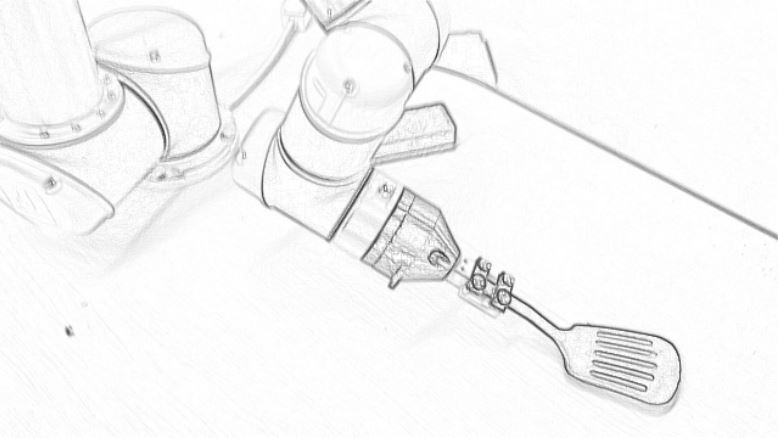
\includegraphics[width=0.60\textwidth]{images/test_image}
\end{figure}
\vspace{0.5 in}
{\centering \huge \color{accentcolor} \sc \textbf{\teamname \\ \productname} \par}
\vspace{0.5 in}
{\centering \large \sc \textbf{\authors} \par}
\newpage


%\vspace{1 in}
%\centerline{January 13th, 2012}
%\newpage

%%% Revision History
\begin{versionhistory}
  	\vhEntry{0.1}{10.02.2017}{LV}{Creating document. Clear up place holder. Add statements to section 1, 2, 3, 7, 8, 10}
  	\vhEntry{0.2}{10.02.2017}{JM}{Add and edit statements of 1, 2, 3, 4, 7, 8, 10}
  	\vhEntry{0.2}{10.02.2017}{JM}{Modifications}
  	\vhEntry{0.3}{5.9.2018}{TB}{Final Draft}
\end{versionhistory}
\newpage

%%% Table of contents
\tableofcontents
\newpage

%%% List of figures and tables (optional)
\listoffigures
%\listoftables
\newpage

%%% Agile project charter sections
\section{Vision}
Our vision for \productname{} is to develop an application for our technology capable of eliminating human involvement in mundane and repetitive tasks, allowing companies to cut down on labor costs and focus more of their attention on complex issues.\\
\\
One specific application of this technology that we have in mind is automating the preparation of grill cheese sandwiches.
\section{Mission}
\input{tex/mission}
\section{Success Criteria}
Ideally, our success criteria will be a successful and robust application of our \productname{} technology. However, due to time constraints and complex college schedules, we will be using the NASA (and Agile) approach to delivering this product successfully. 

Each increment of the product will accomplish a different task and yield a demonstrable product, each one building upon the previous. Even if the end goal product is not delivered, there will still be numerous smaller successes along the way, each with inherent and obvious value.

By the end of the project we will have produced an interface that can handle multiple applications. Whether the application of the product is great in magnitude will be left to the amount of available time to deliver.
\newpage

%%% Remaining project charter sections
\section{Background}
The University of Texas at Arlington has supplied Team Tassium with a state of the art UR5 robotic arm and funding to purchase and develop hardware for the device.

Our team will be focused on fleshing out an application of this hardware combined with the robotic arm.
\section{Related Work}
Ultimaker's 3D printers will be used in making of this project in combination with TinkerCAD modeling software for development of hardware components.

Training will also be utilized for further understanding of the proprietary hardware and software of Universal Robotics UR5 robot.
\section{System Overview}
The main architecture of the system involves 4 main systems communicating with each other. The control logic system and UR5 system pass information with each other via the network system through an Ethernet TCP/IP connection.  The UR5 then provides a signal to the mount system allowing for the docking and undocking of various utensils.

\begin{figure}[h!]
	\centering
 	\includegraphics[width=0.60\textwidth]{images/ADS_layers}
 \caption{A simple architectural layer diagram}
\end{figure}

\subsection{Network}
%%%Each layer should be described separately in detail. Descriptions should include the features, functions, critical interfaces %%%and interactions of the layer. The description should clearly define the services that the layer provides. Also include any %%%%conventions that your team will use in describing the structure: naming conventions for layers, subsystems, modules, and data %%%flows; interface specifications; how layers and subsystems are defined; etc.
This layer contains the router that will allow a connection to the UR5.

\subsection{Control}
This layer contains the camera, raspberry pi that will be use to communicate with the UR5.

\subsection{Mount}
This layer contains the mount that will fit the tool into the mount by controlling the magnet.

\subsection{UR5}
This layer contains the UR5 robot arm, the polyscope(interface), and the control box.
\section{Roles \& Responsibilities}
Technical Expert : Anthony Tatowicz
\\Product Owner : Jesse Daniel Mitchell
\\System Architect : Todd Brewer
\\Scrum Master : Linh Vu
\\
\\

\section{Facilities \& Equipment}
\input{tex/facilities_equipment}
\section{Cost Proposal}
\subsection{Preliminary Budget}
800 USD provided by the University of Texas Arlington

\subsection{Current \& Pending Support}
N/A
\section{Documentation \& Reporting}
This section describes the various artifacts that will be generated during the project lifecycle. 

\subsection{Project Charter}
This will be stored in a GitHub repository where all team members will have access.
The charter will be updated upon unanimous agreement among the team.

\subsection{Product Backlog}
Any items that are necessary to complete the product. This will be updated when the team/product owner develops more knowledge throughout the implementation of the project. The Product Owner will be responsible for adding items to the Product Backlog. 

The Product Owner will be able to approve a feature another team member presents. The Product Owner must have the approval of at least one other member to add a new feature to the product backlog. The Product Owner can be outvoted by the other three team members if they unanimously agree.  

Removal of a feature requires the approval of two other team members (however, the current Scrum Master could alternatively just never assign it).

\subsection{Sprint Planning}
Sprint planning for the next Sprint will be in a group meeting within the last week of another sprint. Plans will be updated if there are any changes that require the team attention.

The Scrum Master will be in charge of approving which items are taken from the Product Backlog for each individual Sprint. He can only overrided if the other three team members unanimously agree.

\subsubsection{Sprint Goal}
The goal of each sprint is to successfully accomplish the main task of that sprint. This will be set and pushed by the Scrum Master, in accordance with the class's current goals.

\subsubsection{Sprint Backlog}
The Sprint backlog will hold the tasks for the current Sprint, which will be pulled from the Product Backlog. 

The Scrum Master will pull items from the Product Backlog for each sprint. The Scrum Master is unable to add new items without approval from the Product Owner.

\subsubsection{Task Breakdown}
Tasks will be distributed to team members when they are clearly defined. They will be posted on a digital Scrum Board where the team members will be allowed to assign themselves to the tasks. 

The Scrum Master is allowed to determine if a task requires more than one team member. The Scrum Master will also be allowed to remove a team member from a task if he is under performing.

If a task is currently unassigned, the Scrum Master is allowed to assign a team member accordingly.

\subsection{Sprint Burndown Charts}
WIP

\begin{figure}[h!]
    \centering
    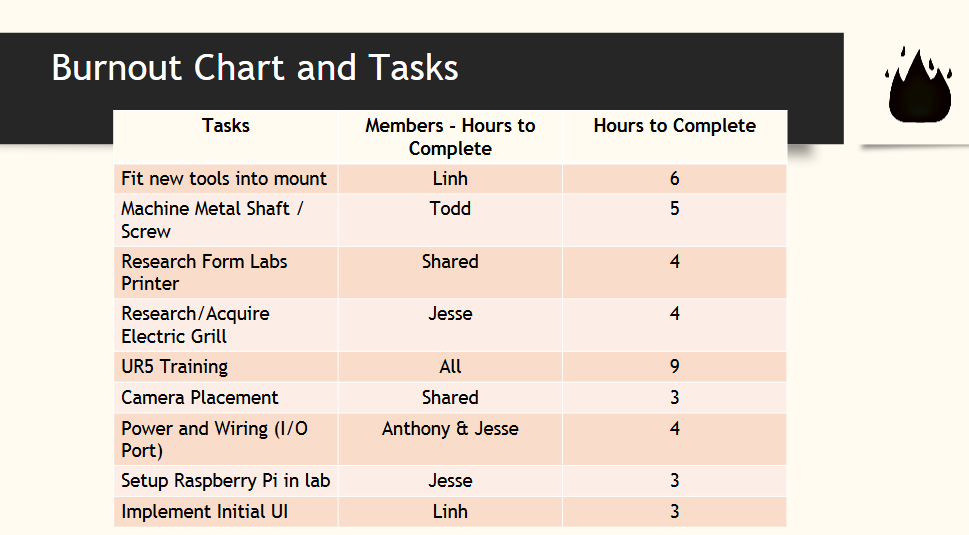
\includegraphics[width=0.5\textwidth]{images/Burndown_Chart}
    \caption{Example sprint burndown chart}
\end{figure}

\subsection{Sprint Retrospectives}
At the end of each sprint the team will be responsible for coming up with a retrospective for the Sprint to analyze what changes should be made for future sprints.

\subsection{Individual Status Reports}
N/A

\subsection{Engineering Notebooks}
Engineering Notebooks will be kept up to date and signed at the end of each week. If no additions are made to the Engineering notebooks, no signatures will be made.

\subsection{Closeout Materials}
The final documents that will be submitted will include this (Project Charter), the System Requirements Specification (SRS), the Architectural Design Specification (ADS), the Detailed Design Specification (DDS), and our Project Poster.

\subsubsection{System Prototype}
System Prototype images are provided at \url{https://goo.gl/d9Fj9v}

\subsubsection{Project Poster}
Project Poster file is provided at \url{https://goo.gl/d9Fj9v}

\subsubsection{Web Page}
Webpage is provided at \url{https://goo.gl/d9Fj9v}

\subsubsection{Demo Video}
Demo Video is provided at \url{https://goo.gl/d9Fj9v}

\subsubsection{Source Code}
Source Code is provided at \url{https://github.com/boomchakalakaZ/UR5}

\subsubsection{Source Code Documentation}
Source Code documentation is provided at \url{https://github.com/boomchakalakaZ/UR5}

\subsubsection{Hardware Schematics}
N/A

\subsubsection{CAD files}
CAD model files (in .stl file format) are provided at \url{https://goo.gl/d9Fj9v}

\subsubsection{Installation Scripts}
N/A

\subsubsection{User Manual}
User Manual for UR5 is provided at \url{https://www.universal-robots.com/media/8704/ur5_user_manual_gb.pdf}
\newpage

%%% References
\bibliographystyle{plain}
\bibliographystyle{reference/IEEEtran_custom}
\bibliography{reference/refs}{}

\end{document}